\chapter*{Appendix: Additional Functional Requirements\\ and Business Logic Model (2018)}
\label{appendix}

\vspace{-1cm}
\begin{center}
Eduard Hirsch and Paolo Dini
\end{center}

In order to see how to manage a more challenging use case based on reading historic data placed on the chain, we model the ``delta-debt'' function as an additional requirement. This example could help foresee possible challenges for more complex tasks. The implementation details for the other requirements covered can be found in D3.2 \cite{INTERLACE_D32}.

\section{Requirement: Debt Record Tracking}

Sardex sets the credit line of the circuit's SME users based on their turnover as well as on their track record. Thus, the balance of an account, as described in the requirements specification deliverables D2.1 and D3.1 \cite{INTERLACE_D21,INTERLACE_D31}, can go negative (with a 0\% interest rate) up to a maximum amount that varies for each member company. It is a Sardex contractual requirement that such a negative amount or debt be ``paid back'' within 12 months of when it was incurred. The debt is not towards Sardex S.p.A. (Sardex S.p.A. is not a bank) and it is not bilateral towards a single other member. Rather, the debt is towards the circuit as a whole. Therefore, the indebted company can pay back or recover its debt simply by selling its products and services to any other members, at least for the amount of the debt and within 12 months of incurring it -- more generally, from the time of each and every transaction that increases the debt of an already negative balance.

More precisely, any transaction that increases the debt of an account triggers a recording of that newly created portion of debt and causes the system to allocate a separately handled due date 12 months later for its repayment. On the other hand, if an account receives a positive amount of credits (due to the sale of a product or service), then the ``debt-portions'' which that account may have accrued up to then are paid back in sequence, starting from the oldest unpaid one.

\renewcommand{\thefigure}{A.\arabic{figure}}
\setcounter{figure}{0}

\begin{figure}[htbp]
  \centering
  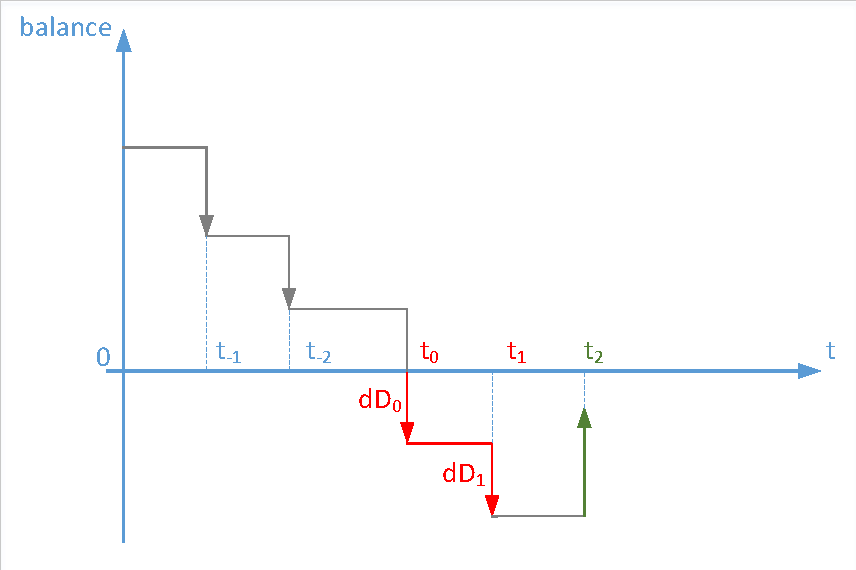
\includegraphics[width=0.7\textwidth, clip, trim=1mm 1mm 1mm 1mm]{Figures/deltadebt}
  \caption{\bf\small The delta-debt progression}
  \label{fig:debt-graph}
\end{figure}

Figure \ref{fig:debt-graph} illustrates a transaction flow for a single account with 5 transactions and their timestamps named $t_i$, where $i$ covers the interval $[-2,2]$ in discrete steps of $1$. Two timestamps $t_j$ and $t_k$ having a $j>k$ imply that $t_j$ is older than $t_k$. Let's assume a transaction at $t_0$, as illustrated in the figure, which turns a positive balance into a negative value. That event then defines a starting timestamp at $t_0$.

This transaction at $t_0$ creates a debt whose value is recorded in the variable $balance$ reduced by the transaction $amount$ given that $balance \ge 0$ and $amount > balance$.

The debts $debt_{t_0}$ and $debt_{t_1}$ created by this transaction and by a possible further transaction, respectively, are represented in Figure \ref{fig:debt-graph}. Debt will be handled further as a positive value, thus, we define a debt created at $t_i$ as

\vspace{0.2cm}
\begin{asm}
	debt_{t_i} = \left\{\begin{array}{ll}
           |balance_{t_i} - amount_{t_i}| \+\+ & \IF i = 0 \AND balance_{t_0} \ge 0 \AND amount > balance\\
           amount_{t_i} & \ELSEIF i > 0 \AND balance_{t_i} < 0\\
           0 & \ELSE
        \end{array}\right.
\end{asm}
\vspace{-0.2cm}

By declaring $txid_{t_i}$ as the id for a transaction which is executed at time $t_i$ and with $accid$ as the account id, we are defining a so-called \textit{deltaDebt} with index $i$ as the following tuple:

\begin{align}
	deltaDebt_i = (t_i, txid_{t_i}, amount_{t_i}, debtPos_{t_i}, accid),
\end{align}

where the $amount_{t_i}$ as well as $debtPos_{t_i}$ are both initialized with $debt_{t_i}$. In the following, $amount_{t_i}$ will always stay with its original value whereas $debtPos_{t_i}$ is reduced by any amount \textbf{received} by the same account.

The creation of a \textit{deltaDebt} can be described as follows:

\begin{asm}
	\ASM{CreateDeltaDebt}(txid,currentDate,from,amount)=\+
		\LET balance = \ASM{balanceOf}(from)\+
			\IF (balance - amount) < 0 \THEN\+
				\LET debt =  \+\left\{\begin{array}{ll}
						|balance - amount|\+& \IF balance > 0\\
						amount & \ELSE
					\end{array}\right.\-\-
				\LET deltaDebt = (currentDate, txid, debt, debt, from)\+
					\ASM{WriteDeltaDebt}(deltaDebt)
\end{asm}

In order to pay back an open debt, at every transfer the $deltaDebt$s need to be checked for possible clearances:

\begin{asm}
	\ASM{ClearDeltaDebt}(txid,to,amount)=\+
		\LET openDeltas = \ASM{SelectOpenDeltaDebtsFor}(to)\+
			\ASM{ClearDebt}(openDeltas, amount)\dec\-
	\WHERE \+
		\ASM{ClearDebt}(openDeltas, amount) =\+
		\IF amount > 0 \THEN\+
			\LET Tmin = \ASM{SelectOldestDebt}(openDeltas)\\
			\IF (Tmin\ \neq\ \UNDEF) \THEN\+
				\IF debtPos(Tmin) \ge amount \THEN\+
					debtPos(Tmin) := debtPos(Tmin) - amount\-
				\ELSE\+
					\LET restAmount = amount - debtPos(Tmin)\+
						debtPos(Tmin) := 0\\
						\ASM{ClearDebt}(\{d \in openDeltas\ |\ d \neq Tmin \}, restAmount )\dec\dec\dec\-
\end{asm}


In this ASM example we assume that \ASM{SelectOpenDeltaDebtsFor} is returning a list of open \textit{deltaDebt} entries from the persistence layer where $debtPos$ of each $deltaDebt$ is bigger than $0$. \ASM{SelectOldestDebt} selects the $deltaDebt$ of a corresponding list that has the minimum timestamp. Further \ASM{SelectOldestDebt} returns \textbf{undef} if $openDeltas$ are empty or also \textbf{undef}.

$debtPos(Tmin)$ reads or writes the pending amount for a particular $deltaDebt$ (here: $Tmin$).









